 %===============================================================================
% LaTeX sjabloon voor de bachelorproef toegepaste informatica aan HOGENT
% Meer info op https://github.com/HoGentTIN/latex-hogent-report
%===============================================================================

\documentclass[english,dit,thesis]{hogentreport}

% TODO:
% - If necessary, replace the option `dit`' with your own department!
%   Valid entries are dbo, dbt, dgz, dit, dlo, dog, dsa, soa
% - If you write your thesis in English (remark: only possible after getting
%   explicit approval!), remove the option "dutch," or replace with "english".

\usepackage{lipsum} % For blind text, can be removed after adding actual content

%% Pictures to include in the text can be put in the graphics/ folder
\graphicspath{{../graphics/}}

%% For source code highlighting, requires pygments to be installed
%% Compile with the -shell-escape flag!
%% \usepackage[chapter]{minted}
%% If you compile with the make_thesis.{bat,sh} script, use the following
%% import instead:
\usepackage[chapter,outputdir=../output]{minted}
\usemintedstyle{solarized-light}
\usepackage{tabularx}

%% Formatting for minted environments.
\setminted{%
    autogobble,
    frame=lines,
    breaklines,
    linenos,
    tabsize=4
}

%% Ensure the list of listings is in the table of contents
\renewcommand\listoflistingscaption{%
    \IfLanguageName{dutch}{Lijst van codefragmenten}{List of listings}
}
\renewcommand\listingscaption{%
    \IfLanguageName{dutch}{Codefragment}{Listing}
}
\renewcommand*\listoflistings{%
    \cleardoublepage\phantomsection\addcontentsline{toc}{chapter}{\listoflistingscaption}%
    \listof{listing}{\listoflistingscaption}%
}

% Other packages not already included can be imported here

%%---------- Document metadata -------------------------------------------------
% TODO: Replace this with your own information
\author{Tristan Van Speybroeck}
\supervisor{Mevr. K. Samyn}
\cosupervisor{Dhr. B. Oloeriu}
\title[]%
    {Automatic technical feedback on the gymnastics skill
        ``kip on bars'' \\ through video analysis
        and Large Language Models}
\academicyear{\advance\year by -1 \the\year--\advance\year by 1 \the\year}
\examperiod{1}
\degreesought{\IfLanguageName{dutch}{Professionele bachelor in de toegepaste informatica}{Bachelor of applied computer science}}
\partialthesis{false} %% To display 'in partial fulfilment'
%\institution{Internshipcompany BVBA.}

%% Add global exceptions to the hyphenation here
\hyphenation{back-slash}

%% The bibliography (style and settings are  found in hogentthesis.cls)
\addbibresource{bachproef.bib}            %% Bibliography file
\addbibresource{../voorstel/voorstel.bib} %% Bibliography research proposal
\defbibheading{bibempty}{}

%% Prevent empty pages for right-handed chapter starts in twoside mode
\renewcommand{\cleardoublepage}{\clearpage}

\renewcommand{\arraystretch}{1.2}

%% Content starts here.
\begin{document}

%---------- Front matter -------------------------------------------------------

\frontmatter

\hypersetup{pageanchor=false} %% Disable page numbering references
%% Render a Dutch outer title page if the main language is English
%\IfLanguageName{english}{%
    %% If necessary, information can be changed here
   % \degreesought{Professionele Bachelor toegepaste informatica}%
  %  \begin{otherlanguage}{dutch}%
 %      \maketitle%
%    \end{otherlanguage}%
%}{}

%% Generates title page content
\maketitle
\hypersetup{pageanchor=true}

%%=============================================================================
%% Voorwoord
%%=============================================================================

\chapter*{\IfLanguageName{dutch}{Woord vooraf}{Preface}}%
\label{ch:voorwoord}

%% TODO:
%% Het voorwoord is het enige deel van de bachelorproef waar je vanuit je
%% eigen standpunt (``ik-vorm'') mag schrijven. Je kan hier bv. motiveren
%% waarom jij het onderwerp wil bespreken.
%% Vergeet ook niet te bedanken wie je geholpen/gesteund/... heeft
This bachelor thesis focuses on automatic technical feedback on the kip on bars through video analysis and Large Language Models. I chose this topic because I personally enjoy sports and find it interesting how technology can support athletes and coaches. Gymnastics is also a sport that I find technically very impressive. The combination of movement, timing, strength and control made the kip on bars an interesting skill for me to investigate further.

The process was not always straightforward. Some ideas turned out to be technically more difficult than expected, and certain results were less strong than hoped. However, these limitations helped to make the proof-of-concept more realistic and better defined.

I would like to thank my supervisor, Ms. K. Samyn, for the regular feedback and guidance throughout this process. Her comments helped me to further refine my bachelor thesis each time and gave me renewed motivation to continue working during difficult moments. I would also like to thank my co-supervisor, Mr. B. Oloeriu, for his guidance and support during this process.

In addition, I would like to thank the gymnasts and coaches of OTV Nazareth for their cooperation. Thanks to the provided video footage, the proof-of-concept could be tested on real executions of the kip on bars. In particular, I would like to thank the coach who helped provide the video material and who gave feedback on parts of my bachelor thesis based on her gymnastics experience.

I would also like to thank Tom Drijvers, my colleague during the internship, for proofreading parts of my bachelor thesis and for the additional feedback. Finally, I would like to thank everyone who supported, helped or motivated me during this period.

For me, this bachelor thesis forms a first exploration of how AI and video analysis can contribute to sport-technical support. I hope that this work can form a useful basis for further research within this domain.
```


%%=============================================================================
%% Samenvatting
%%=============================================================================

% TODO: De "abstract" of samenvatting is een kernachtige (~ 1 blz. voor een
% thesis) synthese van het document.
%
% Een goede abstract biedt een kernachtig antwoord op volgende vragen:
%
% 1. Waarover gaat de bachelorproef?
% 2. Waarom heb je er over geschreven?
% 3. Hoe heb je het onderzoek uitgevoerd?
% 4. Wat waren de resultaten? Wat blijkt uit je onderzoek?
% 5. Wat betekenen je resultaten? Wat is de relevantie voor het werkveld?
%
% Daarom bestaat een abstract uit volgende componenten:
%
% - inleiding + kaderen thema
% - probleemstelling
% - (centrale) onderzoeksvraag
% - onderzoeksdoelstelling
% - methodologie
% - resultaten (beperk tot de belangrijkste, relevant voor de onderzoeksvraag)
% - conclusies, aanbevelingen, beperkingen
%
% LET OP! Een samenvatting is GEEN voorwoord!

%%---------- Nederlandse samenvatting -----------------------------------------
%
% TODO: Als je je bachelorproef in het Engels schrijft, moet je eerst een
% Nederlandse samenvatting invoegen. Haal daarvoor onderstaande code uit
% commentaar.
% Wie zijn bachelorproef in het Nederlands schrijft, kan dit negeren, de inhoud
% wordt niet in het document ingevoegd.

\IfLanguageName{english}{%
\selectlanguage{dutch}
\chapter*{Samenvatting}
\lipsum[1-4]
\selectlanguage{english}
}{}

%%---------- Samenvatting -----------------------------------------------------
% De samenvatting in de hoofdtaal van het document

\chapter*{\IfLanguageName{dutch}{Samenvatting}{Abstract}}

Dit onderzoek gaat na in welke mate een AI-gebaseerd systeem op basis van mark\-er\-loze video-analyse technisch bruikbare feedback kan genereren voor recreatieve turnsters bij de kip aan de barre. Binnen recreatieve gymnastiekclubs begeleiden trainers vaak meerdere turnsters tegelijk, waardoor technische fouten niet altijd systematisch worden opgemerkt. Tegelijk is gerichte feedback belangrijk om de uitvoering van complexe elementen veilig en efficiënt aan te leren.

Het doel van dit onderzoek is het ontwikkelen en verkennend evalueren van een proof-of-concept dat standaard videobeelden omzet naar pose-data, daaruit relevante gewrichtshoeken berekent, vooraf gedefinieerde technische fouten regelgebaseerd detecteert en deze detecties omzet naar tekstuele feedback via een Large Language Model. De nadruk ligt daarbij niet op een volledig gevalideerd coachesysteem, maar op de technische haalbaarheid en beperkingen van een dergelijke analysepipeline.

De proof-of-concept werd opgebouwd in verschillende stappen. Eerst werd Media\-Pipe Pose Landmarker gebruikt om lichaamslandmarks uit videobeelden te extraheren. Vervolgens werden op basis van deze landmarks de heuphoek, schouderhoek, romphoek en ellebooghoek berekend en opgeslagen in CSV-formaat. Daarna werd een Python-script ontwikkeld dat een manueel gekozen analysevenster verwerkt, kritieke ankerpunten detecteert, de beweging opdeelt in fasen en vier vooraf bepaalde fouttypes analyseert: gebogen armen, onvoldoende heupsluiting, te vroege heupopening en onvoldoende schouderdruk in de steunfase. De analyse-output werd gestructureerd opgeslagen in JSON-formaat en in gefilterde vorm gebruikt als input voor een lokale LLM via Ollama.

Uit de resultaten blijkt dat markerloze pose-estimatie bruikbare bewegingsdata kan opleveren uit standaard videobeelden, maar dat de kwaliteit afhankelijk blijft van de opname. Achtergrondbewegingen, tijdelijk minder zichtbare lich\-aams\-delen en detectieruis kunnen abrupte afwijkingen veroorzaken in de berekende hoekcurves. Daarom werd de analyse iteratief verfijnd, onder meer door smoothing toe te passen en foutregels aan te passen om foutieve detecties te beperken.

De finale analyse werd getest op drie pogingen: één goede uitvoering en twee foutieve uitvoeringen. Bij de goede uitvoering werden geen fouten gedetecteerd. Bij de eerste foutieve uitvoering werden gebogen armen in de trekfase en onvoldoende schouderdruk in de steunfase vastgesteld. Bij de tweede foutieve uitvoering werd vooral onvoldoende schouderdruk in de steunfase gedetecteerd. De resultaten tonen aan dat de regelgebaseerde aanpak binnen de beperkte testset relevante verschillen tussen pogingen kan herkennen, maar niet als formele validatie mag worden beschouwd.

De LLM-feedback bleek technisch haalbaar, maar niet volledig betrouwbaar zonder strikte afbakening. Wanneer het taalmodel te veel informatie kreeg, bestond het risico dat het niet-gedetecteerde fouten of algemene verbeterpunten formuleerde. Daarom werd de LLM-input beperkt tot de effectief gedetecteerde fouten en wordt geen LLM-call uitgevoerd wanneer het regelgebaseerde systeem geen fouten detecteert.

Dit onderzoek toont aan dat automatische technische feedback op de kip aan de barre in beperkte mate haalbaar is via een combinatie van markerloze pose-estimatie, regelgebaseerde foutdetectie en LLM-gebaseerde tekstgeneratie. De aanpak biedt potentieel als ondersteunend hulpmiddel voor trainers, maar vervangt geen menselijke expertise. Verdere evaluatie op een grotere dataset en met feedback van ervaren coaches blijft noodzakelijk.


%---------- Inhoud, lijst figuren, ... -----------------------------------------

\tableofcontents

% In a list of figures, the complete caption will be included. To prevent this,
% ALWAYS add a short description in the caption!
%
%  \caption[short description]{elaborate description}
%
% If you do, only the short description will be used in the list of figures

\listoffigures

% If you included tables and/or source code listings, uncomment the appropriate
% lines.
\listoftables

\listoflistings

% Als je een lijst van afkortingen of termen wil toevoegen, dan hoort die
% hier thuis. Gebruik bijvoorbeeld de ``glossaries'' package.
% https://www.overleaf.com/learn/latex/Glossaries

%---------- Kern ---------------------------------------------------------------

\mainmatter{}

% De eerste hoofdstukken van een bachelorproef zijn meestal een inleiding op
% het onderwerp, literatuurstudie en verantwoording methodologie.
% Aarzel niet om een meer beschrijvende titel aan deze hoofdstukken te geven of
% om bijvoorbeeld de inleiding en/of stand van zaken over meerdere hoofdstukken
% te verspreiden!

%%=============================================================================
%% Inleiding
%%=============================================================================

\chapter{\IfLanguageName{dutch}{Inleiding}{Introduction}}%
\label{ch:inleiding}

Artistieke gymnastiek is een technisch veeleisende sport waarbij coördinatie, kracht, mobiliteit en timing goed op elkaar afgestemd moeten worden. Zelfs eenvoudige bewegingen vereisen een correcte uitvoering om efficiënt en veilig uitgevoerd te worden. Binnen recreatieve contexten worden gymnasten regelmatig geconfronteerd met complexe elementen waarvoor zij nog onvoldoende lichaamscontrole of kracht hebben ontwikkeld. Hierdoor ontstaan vaak technische uitvoeringsfouten.

De kip aan barre is een belangrijk overgangselement binnen de damesgymnastiek. Het element vereist een combinatie van zwaaimomentum, heupsluiting, armstrekking en actieve schouderwerking om vanuit hangpositie tot steun op de barre te komen. Vooral bij recreatieve turnsters blijkt deze beweging technisch uitdagend. Dit leidt regelmatig tot fouten zoals gebogen armen, onvoldoende heupsluiting of onvoldoende schouderdruk.

Een correcte technische uitvoering is niet alleen belangrijk voor prestatieverbetering, maar ook voor blessurepreventie. Herhaaldelijk uitvoeren van foutieve bewegingspatronen kan bijdragen aan overbelastingsletsels, vooral ter hoogte van schouder en pols bij bewegingen aan de barre. Het vroegtijdig detecteren en corrigeren van technische fouten is daarom belangrijk binnen een veilige trainingsomgeving.

Binnen recreatieve gymnastiekclubs worden technische elementen meestal in groepsverband aangeleerd. Trainers begeleiden meerdere sporters tegelijk, waardoor er beperkte tijd is voor een grondige individuele analyse van elke uitvoering. Feedback gebeurt voornamelijk op basis van visuele observatie en ervaring van de coach. Geavanceerde 3D bewegingsanalysesystemen bestaan, maar vereisen gespecialiseerde apparatuur en zijn meestal financieel niet haalbaar voor recreatieve clubs. Er is dus een duidelijke kloof tussen laboratoriumgebaseerde bewegingsanalyse en de praktische realiteit in de trainingszaal.

Recente ontwikkelingen in markerloze pose-estimatie maken het mogelijk om gewrichtsposities te bepalen op basis van standaard videobeelden, zonder gebruik van sensoren of markers. Daarnaast kunnen Large Language Models (LLM’s) informatie omzetten in begrijpelijke tekstuele feedback. De combinatie van deze technologieën biedt mogelijkheden voor het ontwikkelen van een laagdrempelig AI-gebaseerd ondersteuningssysteem voor technische analyse in recreatieve gymnastiek.

Deze bachelorproef onderzoekt in welke mate een dergelijk systeem haalbaar en bruikbaar is voor het genereren van technische feedback bij de kip aan barre.

\section{\IfLanguageName{dutch}{Probleemstelling}{Problem Statement}}%
\label{sec:probleemstelling}
Binnen recreatieve en laagcompetitieve gymnastiekclubs worden technische elementen zoals de kip aan barre aangeleerd aan turnsters van ongeveer 10 jaar en ouder. In deze context beschikken clubs doorgaans niet over gespecialiseerde bewegingsanalyseapparatuur en zijn trainers aangewezen op visuele observatie.

De doelgroep van dit onderzoek bestaat uit:

\begin{itemize}
    \item Recreatieve en laagcompetitieve turnsters
    \item Trainers binnen recreatieve gymnastiekclubs
    \item Gymnastiekclubs zonder toegang tot gespecialiseerde bewegingsanalyse
\end{itemize}

Voor deze doelgroep kan een laagdrempelig video-gebaseerd analysesysteem een meerwaarde bieden door:

\begin{itemize}
    \item Consistente detectie van vooraf gedefinieerde technische fouten
    \item Ondersteuning van trainers bij het formuleren van gerichte feedback
    \item Verhoogd bewustzijn van uitvoeringskwaliteit bij sporters
\end{itemize}

De centrale uitdaging bestaat erin te onderzoeken of een AI-gebaseerde oplossing op basis van standaard videobeelden een haalbare en bruikbare ondersteuning kan vormen binnen deze recreatieve trainingscontext.

\section{\IfLanguageName{dutch}{Onderzoeksvraag}{Research question}}%
\label{sec:onderzoeksvraag}
De centrale onderzoeksvraag luidt als volgt:

\textit{In welke mate kan een AI-gebaseerd systeem op basis van markerloze video-analyse technisch bruikbare feedback genereren voor recreatieve turnsters bij de kip aan barre?}

 Om deze onderzoeksvraag te beantwoorden worden volgende deelvragen onderzocht. Deze hebben enerzijds betrekking tot het probleemdomein en anderzijds tot het oplossingsdomein.
\newline
\textbf{Probleemdomein}:

\begin{enumerate}
    \item Welke technische fouten komen het vaakst voor bij de kip?
    \item Waarom worden terugkerende technische fouten door coaches soms niet opgemerkt, en hoe kan dit systematisch worden vastgelegd?
    \item Welke kenmerken maken technische feedback effectief en bruikbaar voor recreatieve turnsters?
\end{enumerate}

\textbf{Oplossingsdomein}:

\begin{enumerate}
    \item Welke markerloze pose-estimatie methode is het meest geschikt voor het analyseren van de kip aan barre binnen een recreatieve trainingscontext?
    \item In welke mate kunnen technische fouten automatisch worden gedetecteerd op basis van pose-data?
    \item In hoeverre kan een Large Language Model technisch correcte en bruikbare feedback geven op basis van gedetecteerde fouten?
    \item Wat zijn de beperkingen van een AI-gebaseerd feedbacksysteem binnen deze toepassing?
\end{enumerate}

\section{\IfLanguageName{dutch}{Onderzoeksdoelstelling}{Research objective}}%
\label{sec:onderzoeksdoelstelling}
Het doel van deze bachelorproef is het ontwikkelen en evalueren van een proof-of-concept van een AI-gebaseerd systeem dat:

\begin{enumerate}
    \item Gewrichtsposities extraheert uit 2D videobeelden via markerloze pose-estimatie.
    \item Vier frequent voorkomende technische fouten bij de kip aan barre rule-based detecteert:
    \begin{itemize}
        \item Gebogen armen tijdens de trekfase
        \item Onvoldoende heupsluiting
        \item Te vroege heupopening
        \item Onvoldoende schouderdruk in steunfase
    \end{itemize}
    \item Gedetecteerde fouten omzet in gestructureerde parameters.
    \item Op basis van deze parameters via een Large Language Model begrijpelijke en gerichte technische feedback genereert.
\end{enumerate}

Daarnaast wordt verkennend onderzocht in welke mate de geselecteerde fouttypes detecteerbaar zijn via 2D pose-estimatie en of de gegenereerde feedback inhoudelijk aansluit bij de gedetecteerde fouten.

Het onderzoek richt zich op de technische haalbaarheid en praktische bruikbaarheid binnen een recreatieve context, en niet op de ontwikkeling van een volledig gevalideerd diagnostisch systeem.

\section{\IfLanguageName{dutch}{Opzet van deze bachelorproef}{Structure of this bachelor thesis}}%
\label{sec:opzet-bachelorproef}

% Het is gebruikelijk aan het einde van de inleiding een overzicht te
% geven van de opbouw van de rest van de tekst. Deze sectie bevat al een aanzet
% die je kan aanvullen/aanpassen in functie van je eigen tekst.

De rest van deze bachelorproef is als volgt opgebouwd:

In Hoofdstuk~\ref{ch:stand-van-zaken} wordt een overzicht gegeven van de stand van zaken binnen het onderzoeksdomein, op basis van een literatuurstudie.

In Hoofdstuk~\ref{ch:methodologie} wordt de methodologie toegelicht en worden de gebruikte onderzoekstechnieken besproken om een antwoord te kunnen formuleren op de onderzoeksvragen.

% TODO: Vul hier aan voor je eigen hoofstukken, één of twee zinnen per hoofdstuk
In Hoofdstuk~\ref{ch:resultaten} worden de implementatie van de proof-of-concept, de regelgebaseerde foutdetectie en de feedbackgeneratie besproken.

In Hoofdstuk~\ref{ch:conclusie}, tenslotte, wordt de conclusie gegeven en een antwoord geformuleerd op de onderzoeksvragen. Daarbij wordt ook een aanzet gegeven voor toekomstig onderzoek binnen dit domein.
\chapter{\IfLanguageName{dutch}{Stand van zaken}{State of the art}}%
\label{ch:stand-van-zaken}

% Tip: Begin elk hoofdstuk met een paragraaf inleiding die beschrijft hoe
% dit hoofdstuk past binnen het geheel van de bachelorproef. Geef in het
% bijzonder aan wat de link is met het vorige en volgende hoofdstuk.

% Pas na deze inleidende paragraaf komt de eerste sectiehoofding.
\section{Techniek en blessurerisico in gymnastiek}
\label{sec:techniek-blessures}
Gymnastiek is een technisch veeleisende sport waarbij hoge belastingen op het lichaam ontstaan. In de praktijk zien we dat de meeste blessures optreden in de onderste ledematen, met name enkels (verstuikingen) en knieën, terwijl bij mannen vaker de bovenste extremiteiten (schouders) zijn aangedaan. Zo noteerden \textcite{Hart2018} dat enkels en knieën de meest voorkomende blessurelocaties zijn, terwijl bij mannelijke turners schouderletsels domineren. Uit systematische analyses (Thomas & Thomas, 2019) blijkt dat meer dan de helft van alle turnblessures zich in het onderlichaam voordoet, voornamelijk aan enkels en knieën~\autocite{Thomas2019}. De bijzondere aard van gymnastiek – waarbij gymnasten zich herhaaldelijk op handen en armen landen leidt tot specifieke overbelastingsletsels, stressfracturen en groeischijfletsels van de pols zijn bekende voorbeelden die onder de verzamelnaam “gymnast’s wrist” vallen. \textcite{Concannon2020} onderschrijft dit, zij rapporteren dat bij vrouwelijke gymnasten polsblessures vaker voorkomen, terwijl mannelijke gymnasten relatief meer schouderproblemen kennen.
\newline
\newline
Techniek speelt een cruciale rol in deze blessurepatronen. Harde landingen en elementen als handsprings en salto’s genereren extreem hoge krachten. \textcite{Hart2018} noemen specifiek dat voorwaartse en achterwaartse handsprings en salto’s de meest blessureveroorzakende oefeningen zijn. Biomechanische studies bevestigen dat kleine aanpassingen in techniek het letselrisico kunnen beïnvloeden. Zo vonden \textcite{FARANA201588} dat het uitvoeren van een rond-off met een ‘T-vormige’ handplaatsing resulteert in lagere piekbelastingen en valversnellingen in de elleboog in vergelijking met een parallelle handplaatsing. Deze ‘T-vormige’ techniek reduceert de verticale en anteroposteriore krachten aanzienlijk, wat erop wijst dat een gerichte techniekkeuze effectief letsel kan verminderen. Dergelijke bevindingen illustreren dat techniekkeuzes onmiskenbaar van invloed zijn op gewrichtslast. Tegelijkertijd wijst \textcite{Daly1999HighImpact} erop dat trainingsomgevingen zeer belastend zijn, een turntraining kan gemakkelijk meer dan 100 stuiterende hand-landingen per sessie inhouden. Deze herhaalde impactbelastingen leiden tot cumulatieve microtraumata aan de bovenste extremiteiten, wat chronische overbelastingsletsel in de hand en pols bevordert.
\newline
\newline
Kortom, de combinatie van hoge krachten, herhaalde landingen en complexe bewegingen maakt gymnastiek kwetsbaar voor blessures. Traditionele blessures als enkelverstuikingen en knieverstuikingen wijzen op akoesto-mechanische belasting, terwijl “gymnast’s wrist” en rugproblemen het gevolg zijn van repetitieve overbelasting van unieke houdingen (zoals handstanden). Aangezien veel gymnasten jong zijn en in de groeiperiode trainen, dragen ook groeigerelateerde kwetsbaarheden bij aan deze blessurepatronen~\autocite{Wolf2020,Concannon2020}. Deze bevindingen schetsen het probleemkader, precieze techniekcontrole en tijdige feedback zijn essentieel om blessures te voorkomen, maar in de praktijk blijven coachobservatie en training traditioneel en menselijk. Dit legt de basis voor de noodzaak van geautomatiseerde analyse- en feedbacksystemen in het ontwerp van ons proof-of-concept.

\section{Feedback in motorisch leren}
\label{sec:feedback-motorisch}
Traditionele gymnastiektraining steunt sterk op coachobservatie en directe terugkoppeling. Coaches geven mondelinge aanwijzingen over houding en techniek (kennis van prestaties, KP) en beoordelen de uitkomst (kennis van resultaat, KR)\autocite{Niznikowski2025}. Vaak werkt dit via directe demonstratie, verbale correctie en het gebruik van videoanalyse. Bijvoorbeeld kan een coach turners laten oefenen voor en achter spiegels, of video-opnamen gebruiken om de oefening terug te kijken. Onderzoek wijst uit dat het hanteren van videofeedback een effectief hulpmiddel is. \textcite{Boyer2009} toonden aan dat jongere gymnasten die zowel expertvideo’s als video-opnames van hun eigen uitvoering bekeken, significant sneller en met betere techniek leerden.
\newline
\newline
Naast visuele middelen speelt verbale feedback een belangrijke rol. \textcite{Niznikowski2025} laten zien dat gerichte feedback over kernpunten in de techniek uitermate effectief is. In hun studie kregen gymnasten ofwel feedback over alle fouten, ofwel alleen over de belangrijkste elementen van de oefening. De groep die uitsluitend ‘sleutelelementen’ teruggekoppeld kreeg, behaalden significant hogere scores bij een complexe balanceerbaloefening (de saldana op de balk) vergeleken met de groep die alle fouten hoorde. Hun conclusie is duidelijk, het doseren van feedback, minder frequent en gericht leidt tot betere leerresultaten dan voortdurende, allesomvattende foutencorrectie. Coaches dienen dus strategisch te zijn, het aanwijzen van cruciale bewegingsfouten (bijv. juiste armhoek of lichaamsrotatie) bevordert het leerproces aanzienlijk, in lijn met theorieën in motorisch leren.
\newline
\newline
Deze bevindingen onderstrepen de rol van feedback als leerinstrument, maar ze wijzen ook op knelpunten. De huidige praktijk is afhankelijk van de ervaring en het moment van de coach. Observatie kan worden bemoeilijkt door complexe hoeken of snelle bewegingen die het oog van een coach ontgaan. Bovendien is beoordeling vaak kwalitatief en subjectief, zonder directe kwantificering van de beweging. Deze beperkingen vormen het vertrekpunt voor technische oplossingen. Geautomatiseerde systemen kunnen coaches ondersteunen door objectieve data te leveren over hoekafwijkingen, snelheid of positie. Daarmee kunnen zij aanvullende, gedetailleerde feedback genereren op basis van videobeelden of sensoren, zodat gymnasten direct inzicht krijgen in hun prestatie.

\section{Markerloze pose-estimatie en bewegingsanalyse}
\label{sec:pose-estimatie-bewegingsanalyse}
Markerloze bewegingsanalyse is een technologie waarbij de lichaamspositie van sporters automatisch wordt geschat zonder dat markers of dure sensoren nodig zijn. Traditioneel is voor biomechanische analyse vaak gebruikgemaakt van marker-gebaseerde systemen in laboratoria (met infraroodcamera’s en reflecterende markers), maar deze zijn kostbaar en weinig praktisch voor alledaags gebruik. De recente opkomst van markerloze alternatieven maakt grootschalige analyses in de ‘werkelijkheid’ mogelijk. Zoals \textcite{Ota2025Markerless} beschrijft, omvat markerloze analyse diverse technieken, draagbare IMU-sensoren (accelerometers/gyroscopen), depth-camera’s (bijv. Microsoft Kinect), handmatige digitalisering van video en AI-gebaseerde houdingsschatters. AI-algoritmes (zoals OpenPose of mediapipe) analyseren conventionele videosignalen en berekenen daarmee de posities van gewrichten in 2D of 3D.

\section{Automatische foutdetectie en AI in sportanalyse}
\label{sec:auto-foutdetectie}

\section{Large Language Models en automatische feedbackgeneratie}
\label{sec:LLM-feedback}


%Dit hoofdstuk bevat je literatuurstudie. De inhoud gaat verder op de inleiding, maar zal het onderwerp van de bachelorproef *diepgaand* uitspitten. De bedoeling is dat de lezer na lezing van dit hoofdstuk helemaal op de hoogte is van de huidige stand van zaken (state-of-the-art) in het onderzoeksdomein. Iemand die niet vertrouwd is met het onderwerp, weet nu voldoende om de rest van het verhaal te kunnen volgen, zonder dat die er nog andere informatie moet over opzoeken \autocite{Pollefliet2011}.
%
%Je verwijst bij elke bewering die je doet, vakterm die je introduceert, enz.\ naar je bronnen. In \LaTeX{} kan dat met het commando \texttt{$\backslash${textcite\{\}}} of \texttt{$\backslash${autocite\{\}}}. Als argument van het commando geef je de ``sleutel'' van een ``record'' in een bibliografische databank in het Bib\LaTeX{}-formaat (een tekstbestand). Als je expliciet naar de auteur verwijst in de zin (narratieve referentie), gebruik je \texttt{$\backslash${}textcite\{\}}. Soms is de auteursnaam niet expliciet een onderdeel van de zin, dan gebruik je \texttt{$\backslash${}autocite\{\}} (referentie tussen haakjes). Dit gebruik je bv.~bij een citaat, of om in het bijschrift van een overgenomen afbeelding, broncode, tabel, enz. te verwijzen naar de bron. In de volgende paragraaf een voorbeeld van elk.
%
%\textcite{Knuth1998} schreef een van de standaardwerken over sorteer- en zoekalgoritmen. Experten zijn het erover eens dat cloud computing een interessante opportuniteit vormen, zowel voor gebruikers als voor dienstverleners op vlak van informatietechnologie~\autocite{Creeger2009}.
%
%Let er ook op: het \texttt{cite}-commando voor de punt, dus binnen de zin. Je verwijst meteen naar een bron in de eerste zin die erop gebaseerd is, dus niet pas op het einde van een paragraaf.
%
%\begin{figure}
%  \centering
%  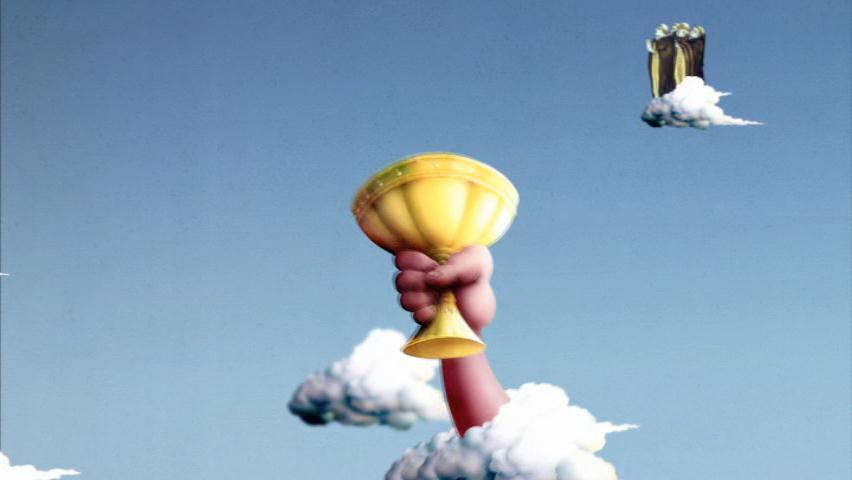
\includegraphics[width=0.8\textwidth]{grail.jpg}
%  \caption[Voorbeeld figuur.]{\label{fig:grail}Voorbeeld van invoegen van een figuur. Zorg altijd voor een uitgebreid bijschrift dat de figuur volledig beschrijft zonder in de tekst te moeten gaan zoeken. Vergeet ook je bronvermelding niet!}
%\end{figure}
%
%\begin{listing}
%  \begin{minted}{python}
%    import pandas as pd
%    import seaborn as sns
%
%    penguins = sns.load_dataset('penguins')
%    sns.relplot(data=penguins, x="flipper_length_mm", y="bill_length_mm", hue="species")
%  \end{minted}
%  \caption[Voorbeeld codefragment]{Voorbeeld van het invoegen van een codefragment.}
%\end{listing}
%
%\lipsum[7-20]
%
%\begin{table}
%  \centering
%  \begin{tabular}{lcr}
%    \toprule
%    \textbf{Kolom 1} & \textbf{Kolom 2} & \textbf{Kolom 3} \\
%    $\alpha$         & $\beta$          & $\gamma$         \\
%    \midrule
%    A                & 10.230           & a                \\
%    B                & 45.678           & b                \\
%    C                & 99.987           & c                \\
%    \bottomrule
%  \end{tabular}
%  \caption[Voorbeeld tabel]{\label{tab:example}Voorbeeld van een tabel.}
%\end{table}


%%=============================================================================
%% Methodologie
%%=============================================================================

\chapter{\IfLanguageName{dutch}{Methodologie}{Methodology}}%
\label{ch:methodologie}

%% TODO: In dit hoofstuk geef je een korte toelichting over hoe je te werk bent
%% gegaan. Verdeel je onderzoek in grote fasen, en licht in elke fase toe wat
%% de doelstelling was, welke deliverables daar uit gekomen zijn, en welke
%% onderzoeksmethoden je daarbij toegepast hebt. Verantwoord waarom je
%% op deze manier te werk gegaan bent.
%% 
%% Voorbeelden van zulke fasen zijn: literatuurstudie, opstellen van een
%% requirements-analyse, opstellen long-list (bij vergelijkende studie),
%% selectie van geschikte tools (bij vergelijkende studie, "short-list"),
%% opzetten testopstelling/PoC, uitvoeren testen en verzamelen
%% van resultaten, analyse van resultaten, ...
%%
%% !!!!! LET OP !!!!!
%%
%% Het is uitdrukkelijk NIET de bedoeling dat je het grootste deel van de corpus
%% van je bachelorproef in dit hoofstuk verwerkt! Dit hoofdstuk is eerder een
%% kort overzicht van je plan van aanpak.
%%
%% Maak voor elke fase (behalve het literatuuronderzoek) een NIEUW HOOFDSTUK aan
%% en geef het een gepaste titel.
Dit onderzoek volgt een ontwerpgericht en experimenteel onderzoeksdesign waarbij een proof-of-concept wordt ontwikkeld en geëvalueerd. Het doel is om na te gaan in welke mate AI-technieken ingezet kunnen worden voor automatische foutdetectie en feedbackgeneratie bij de kip aan barre.

Het onderzoeksproces wordt onderverdeeld in vijf grote fasen.

\section{Fase 1: Literatuurstudie}

In de eerste fase gebeurt een literatuurstudie uitgevoerd rond drie kerncomponenten: 

\begin{itemize}
    \item biomechanische kenmerken van de kip aan barre en veelvoorkomende fouten
    \item markerloze pose-estimatie in sportanalyse
    \item automatische foutdetectie en AI-gebaseerde feedbacksystemen
\end{itemize}

\textbf{Doelstelling:} theoretisch kader opbouwen en technische haalbaarheid inschatten.  

\textbf{Deliverable:} uitgewerkt literatuurhoofdstuk met onderbouwing van de gekozen aanpak.  

\textbf{Onderzoeksmethode:} systematische analyse van wetenschappelijke publicaties en bestaande toepassingen binnen sportanalyse.

\section{Fase 2: Specificatie van fouttypes en systeemvereisten}

\subsection{Specificatie van detecteerbare fouttypes}

Op basis van de literatuur en praktijkervaring binnen recreatieve gymnastiek worden concrete fouttypes gedefinieerd die automatisch detecteerbaar moeten zijn (zoals gebogen armen of onvoldoende heupsluiting).

Daarnaast worden systeemvereisten opgesteld die bepalen welke functionaliteiten het proof-of-concept minimaal moet bevatten. Hierbij wordt expliciet rekening gehouden met de praktische context van recreatieve gymnastiek, waarin gewerkt wordt met standaard videobeelden en beperkte technische infrastructuur.

Naast deze foutdefinities op basis van gewrichtshoeken wordt in de literatuur ook gewezen op het belang van kritieke tussenpunten (via-points) in de beweging \autocite{Yamasaki2010}.

Binnen dit onderzoek worden deze via-points initieel niet expliciet gemodelleerd in de eerste versie van het systeem. In plaats daarvan wordt gekozen voor een vereenvoudigde representatie op basis van fasen en gewrichtshoeken, om de technische haalbaarheid van automatische foutdetectie eerst te valideren.

De integratie van via-points als aanvullende analysemethode wordt voorzien als mogelijke uitbreiding in een iteratieve ontwikkelingsfase.

\subsection{Systeemvereisten}
\subsubsection{Functionele vereisten}

De functionele vereisten beschrijven welke functionaliteiten het systeem moet implementeren om de vooropgestelde doelstelling te bereiken. Voor dit proof-of-concept worden de volgende vereisten gedefinieerd:

\begin{enumerate}
    \item Het systeem moet een videofragment van een kip aan de barre kunnen inladen.
    \item Het systeem moet automatisch gewrichtsposities extraheren uit de video via markerloze pose-estimatie.
    \item Het systeem moet de beweging opdelen in relevante fasen (zwaai, trek, heupsluiting en steunfase).
    \item Het systeem moet vooraf gedefinieerde technische fouten detecteren op basis van pose-data:
    \begin{itemize}
        \item Gebogen armen tijdens de trekfase
        \item Onvoldoende heupsluiting
        \item Te vroege heupopening
        \item Onvoldoende schouderdruk in de steunfase
    \end{itemize}
    \item Het systeem moet de gedetecteerde fouten omzetten naar gestructureerde parameters.
    \item Het systeem moet op basis van deze parameters automatisch tekstuele feedback genereren via een Large Language Model.
    \item Het systeem moet de gegenereerde feedback tonen aan de gebruiker.
\end{enumerate}

\subsubsection{Niet-functionele vereisten}

Naast de functionele vereisten worden ook niet-functionele vereisten gedefinieerd. Deze beschrijven kwaliteitsaspecten waaraan het systeem moet voldoen en worden opgesteld volgens het SMART-principe.

\begin{table}[h]
    \centering
    \begin{tabular}{llll}
        \toprule
        NFR & Indicator & Meetvoorschrift & Norm \\
        \midrule
        Prestatie-efficiëntie & Snelheid & Tijd tussen input video en gegenereerde feedback & $\leq$ 10 s \\
        Functionele geschiktheid & Correctheid & Vergelijking met annotatie door expert & $\geq$ 70\% \\
        Bruikbaarheid & Begrijpelijkheid & Evaluatie door coach (Likert-schaal) & $\geq$ 3/5 \\
        Betrouwbaarheid & Foutbestendigheid & Testen met verschillende video’s & Geen crashes \\
        Overdraagbaarheid & Compatibiliteit & Ondersteunde videoformaten & Minstens MP4 \\
        \bottomrule
    \end{tabular}
    \caption{Niet-functionele vereisten}
\end{table}

\subsection{Prioritering van vereisten (MoSCoW)}

Om de scope van het proof-of-concept duidelijk af te bakenen, worden de vereisten geprioriteerd volgens de MoSCoW-methode.

\textbf{Must have}
\begin{itemize}
    \item Video-invoer
    \item Pose-estimatie
    \item Detectie van de vier gedefinieerde fouttypes
    \item Generatie van tekstuele feedback
\end{itemize}

\textbf{Should have}
\begin{itemize}
    \item Opsplitsing van de beweging in fasen
    \item Structurering van parameters
\end{itemize}

\textbf{Could have}
\begin{itemize}
    \item Visualisatie van het skelet op de video
    \item Vergelijking van meerdere pogingen
\end{itemize}

\textbf{Won't have}
\begin{itemize}
    \item Real-time analyse
    \item Mobiele applicatie
    \item Volledig gevalideerd coachesysteem
\end{itemize}

\textbf{Doelstelling:} afbakenen wat het systeem precies moet detecteren en genereren.  

\textbf{Deliverable:} lijst van fouttypes, systeemvereisten en bijhorende meetbare parameters.  

\textbf{Onderzoeksmethode:} conceptuele analyse en vertaling van biomechanische fouten naar kwantificeerbare bewegingskenmerken.

\section{Fase 3: Exploratief experiment met bestaande AI-systemen}

Voorafgaand aan de ontwikkeling van het proof-of-concept vindt een verkennend experiment plaats uitgevoerd met bestaande Large Language Models (LLMs), met als doel hun huidige capaciteiten voor gymnastiekanalyse te evalueren.

In dit experiment wordt eenzelfde kip-oefening aangeboden aan het model in drie verschillende representaties: (1) ruwe videobeelden, (2) pose-estimatie data in CSV-formaat, en (3) een grafische voorstelling van afgeleide gewrichtshoeken. Voor elk van deze inputvormen wordt een gelijkaardige prompt gebruikt waarbij het model wordt gevraagd om de beweging te analyseren, fasen te identificeren en technische feedback te formuleren.

\textbf{Doelstelling:} inzicht verkrijgen in de mogelijkheden en beperkingen van bestaande AI-systemen voor automatische bewegingsanalyse en feedbackgeneratie.

\textbf{Deliverable:} kwalitatieve analyse van de gegenereerde feedback per inputtype.

\textbf{Onderzoeksmethode:} exploratief experiment waarbij verschillende inputmodaliteiten systematisch worden vergeleken op basis van de gegenereerde output.

\section{Fase 4: Ontwikkeling van een proof-of-concept}

In deze fase wordt een proof-of-concept ontwikkeld waarin videobeelden worden verwerkt via markerloze pose-estimatie. Op basis van de geëxtraheerde keypoints worden relevante hoeken en bewegingsparameters berekend.

De videobeelden worden verwerkt met behulp van een Python-gebaseerde analysepipeline. Hiervoor wordt gebruikgemaakt van het MediaPipe Pose Landmarker model, dat markerloze pose-estimatie uitvoert op RGB-videoframes. Het gebruikte model detecteert per frame lichaamslandmarks die de positie van gewrichten beschrijven.

De gedetecteerde landmarks worden frame per frame geëxtraheerd en opgeslagen, waardoor een tijdreeks van lichaamsposities ontstaat. Op basis van deze gegevens worden bijkomende bewegingskenmerken berekend, zoals gewrichtshoeken. Deze kenmerken vormen de basis voor de verdere analyse van de beweging en de detectie van technische fouten in de kip-oefening.

De foutdetectie gebeurt via een rule-based benadering, waarbij vooraf gedefinieerde drempelwaarden bepalen of een fout aanwezig is. Gezien het exploratieve karakter van dit onderzoek en de beperkte beschikbaarheid van gelabelde trainingsdata wordt bewust gekozen voor een regelgebaseerde benadering in plaats van een volledig data-gedreven machine learning model. Deze aanpak verhoogt de interpreteerbaarheid van het systeem en laat toe om biomechanische criteria expliciet te definiëren.

Hoewel deze regelgebaseerde aanpak voornamelijk focust op drempelwaarden van gewrichtshoeken, sluit dit gedeeltelijk aan bij biomechanische inzichten uit de literatuur. 

Meer geavanceerde modellen, zoals beschreven door \textcite{Yamasaki2010}, suggereren dat bewegingen zoals de kip eerder bepaald worden door kritieke overgangsmomenten (via-points). Binnen dit proof-of-concept wordt echter gekozen voor een vereenvoudigde implementatie, waarbij deze dynamische aspecten impliciet benaderd worden via tijdsafhankelijke veranderingen in gewrichtshoeken.

Binnen de context van dit proof-of-concept vormt deze aanpak een geschikte eerste stap om de technische haalbaarheid van automatische foutdetectie te onderzoeken.

Gedetecteerde fouten worden vervolgens via een Large Language Model omgezet in gestructureerde tekstuele feedback.

Om de output van het systeem te structureren en consistent te maken, wordt een gestandaardiseerd dataformaat gedefinieerd in JSON-vorm. Dit formaat bevat informatie over de geïdentificeerde bewegingsfasen, berekende gewrichtshoeken en gedetecteerde technische fouten.

Deze gestructureerde representatie vormt de interface tussen de rule-based foutdetectie en de feedbackgeneratie via een Large Language Model. Om deze gegevens op een consistente manier door het taalmodel te laten interpreteren, wordt gebruikgemaakt van function calling en een vooraf gedefinieerd JSON-schema. Hierbij wordt het Large Language Model niet aangesproken met vrije tekstinput alleen, maar met een strikt gestructureerde datastructuur waarin per fouttype, bewegingsfase en relevante hoekwaarden expliciete velden zijn voorzien. Function calling laat toe het model te dwingen deze structuur correct te lezen en de output volgens een voorspelbaar formaat op te bouwen. Dit vermindert ambiguïteit in de interpretatie en verhoogt de reproduceerbaarheid van de gegenereerde feedback.

\textbf{Doelstelling:} aantonen dat automatische detectie en feedbackgeneratie technisch haalbaar zijn.  

\textbf{Deliverable:}  een proof-of-concept systeem dat videobeelden analyseert met behulp van pose-estimatie, bewegingskenmerken berekent en op basis daarvan automatische foutdetectie en feedbackgeneratie uitvoert.  

\textbf{Onderzoeksmethode:} experimentele implementatie en iteratieve ontwikkeling.

\section{Fase 5: Evaluatie}

Tot slot wordt het systeem geëvalueerd op twee niveaus: technische detectienauwkeurigheid en bruikbaarheid van de gegenereerde feedback.

De automatische foutdetectie wordt vergeleken met manuele beoordeling door een trainer. De feedbackoutput wordt kwalitatief beoordeeld op technische correctheid en toepasbaarheid binnen een trainingscontext.

Daarnaast wordt geëvalueerd in welke mate de huidige fase- en hoekgebaseerde benadering voldoende is om relevante technische fouten te detecteren, en of een uitbreiding naar een via-point gebaseerde analyse noodzakelijk is.

\textbf{Doelstelling:} inschatten in welke mate het systeem betrouwbaar en pedagogisch bruikbaar is.  

\textbf{Deliverable:} evaluatie-analyse en interpretatie van de resultaten.  

\textbf{Onderzoeksmethode:} vergelijkende analyse en kwalitatieve expertbeoordeling.


%%=============================================================================
%% Resultaten
%%=============================================================================

\chapter{\IfLanguageName{dutch}{Resultaten en proof-of-concept implementatie}{Results and proof-of-concept implementation}}
\label{ch:resultaten}

\section{Implementatie van markerloze pose-estimatie}

De eerste stap in de ontwikkeling van het proof-of-concept bestond uit het automatisch extraheren van lichaamslandmarks uit videobeelden van een gymnast die een kip aan de barre uitvoert. In overeenstemming met de in Hoofdstuk~\ref{ch:stand-van-zaken} besproken markerloze bewegingsanalyse werd hiervoor gebruikgemaakt van het MediaPipe Pose Landmarker model, dat per frame anatomische sleutelpunten van het lichaam detecteert.

In een initiële implementatiefase werd een Python-pipeline ontwikkeld die het videofragment frame per frame verwerkt en voor elk frame de gedetecteerde pose-landmarks teruggeeft. Deze landmarks werden eerst visueel geprojecteerd op het originele videobeeld om na te gaan of de gymnast tijdens de volledige beweging consistent gevolgd werd.

De eerste testresultaten toonden aan dat de globale lichaamsconfiguratie van de uitvoerende gymnast in het merendeel van de frames correct werd gereconstrueerd. De belangrijkste proximale gewrichten, met name schouders, heupen en knieën, bleven voldoende stabiel detecteerbaar tijdens de zwaaifase, de heupsluiting en de uiteindelijke steunfase. Hierdoor bleek de pose-estimatie voldoende bruikbaar als basis voor verdere biomechanische analyse.

Na deze eerste validatie werd de visualisatie uitgebreid met een skeletoverlay waarbij anatomisch verbonden landmarks met elkaar verbonden werden. Deze skeletweergave liet toe om de dynamiek van de lichaamspositie duidelijker te observeren en maakte het eenvoudiger om te controleren of abrupte detectiesprongen effectief overeenkwamen met veranderingen in de beweging.

Een belangrijke praktische bevinding tijdens deze implementatiefase was dat de gebruikte trainingsvideo geen volledig gecontroleerde opname betrof. Op de achtergrond bevond zich bijkomend een tweede turnster die eveneens gedeeltelijk in beeld kwam. In verschillende frames detecteerde het pose-estimatiemodel hierdoor tijdelijk lichaamssegmenten van beide personen binnen dezelfde scène, wat leidde tot verstoringen in de gegenereerde landmarkdata. Deze observatie bevestigt dat markerloze pose-estimatie sterk afhankelijk blijft van de visuele zuiverheid van het inputbeeld en gevoelig is voor aanwezigheid van meerdere personen in het cameraveld, zoals ook in de literatuur wordt aangehaald bij praktijktoepassingen buiten laboratoriumomstandigheden \autocite{Ota2025Markerless}.

Ondanks deze verstoringen bleek de pose-detectie over het volledige videofragment voldoende consistent om verder te gebruiken binnen de proof-of-concept pipeline. De visuele validatie bevestigde dat de kernsegmenten van de uitvoerende gymnast in voldoende mate reconstrueerbaar waren, waardoor een volgende stap mogelijk werd, namelijk het numeriek opslaan van deze pose-data en het afleiden van biomechanisch interpreteerbare gewrichtsparameters.

\section{Extractie en opslag van biomechanische parameters}

Na de visuele validatie van de pose-estimatie werd de pipeline uitgebreid met een numerieke extractiestap waarbij alle gedetecteerde lichaamslandmarks frame per frame automatisch werden opgeslagen in een CSV-bestand. Per videoframe werden voor elke gedetecteerde landmark de genormaliseerde $x$-, $y$- en $z$-coördinaten geregistreerd, waardoor een volledige tijdsreeks van opeenvolgende lichaamshoudingen ontstond.

Deze ruwe pose-data vormde op zichzelf echter nog geen direct interpreteerbare basis voor technische bewegingsanalyse. Om de beweging biomechanisch beschrijfbaar te maken werden bijkomend drie afgeleide gewrichtsparameters geïmplementeerd die aansluiten bij de in Sectie~\ref{sec:Biomechanische-analyse} geïdentificeerde kritieke bewegingscomponenten van de kip:

\begin{itemize}
    \item heuphoek (\textit{schouder--heup--knie}),
    \item schouderhoek (\textit{elleboog--schouder--heup}),
    \item romphoek (\textit{schouder--heup--enkel}).
\end{itemize}

Deze hoeken werden per frame berekend via vectorgeometrie en samen met de ruwe landmarkcoördinaten toegevoegd aan dezelfde CSV-structuur. Hierdoor werd elk videoframe niet enkel gerepresenteerd als een verzameling lichaamsposities, maar ook als een set direct interpreteerbare biomechanische parameters.

Om de invloed van de videokwaliteit en de visuele zuiverheid van de opname op de geëxtraheerde hoekdata verder te beoordelen, werd dezelfde analyse ook uitgevoerd op een tweede videofragment waarin beduidend minder visuele verstoring aanwezig was. In tegenstelling tot de eerste opname, waarin een tweede turnster gedeeltelijk in beeld kwam, bevatte deze tweede opname weinig tot geen storende achtergrondbeweging. Hierdoor kon nagegaan worden in welke mate de eerder vastgestelde fluctuaties in de hoekcurves samenhangen met detectieruis in de pose-estimatie.

Figuur~\ref{fig:jointangles_comparison} vergelijkt het tijdsverloop van de automatisch berekende heup-, schouder- en romphoek voor beide videofragmenten. De bovenste grafiek toont de eerder geanalyseerde opname met duidelijke detectieruis. Hoewel de globale beweging nog herkenbaar blijft, komen op meerdere plaatsen abrupte pieken, scherpe dalingen en kortstondige sprongen voor die biomechanisch moeilijk te verklaren zijn. Een duidelijk voorbeeld hiervan is zichtbaar in het midden en het laatste deel van de tijdsreeks, waar verschillende hoekwaarden plots sterk veranderen over slechts enkele opeenvolgende frames.

De onderste grafiek, afkomstig van de video met weinig visuele ruis, vertoont een merkbaar vloeiender verloop. De evolutie van de heuphoek, schouderhoek en romphoek is consistenter en de grote, abrupte detectiesprongen komen veel minder voor. Hierdoor zijn de bewegingspatronen duidelijker interpreteerbaar. Zo blijft de afname en daaropvolgende heropening van de heuphoek beter zichtbaar, terwijl ook de globale evolutie van de romphoek minder grillig verloopt.

\begin{figure}[h]
    \centering
    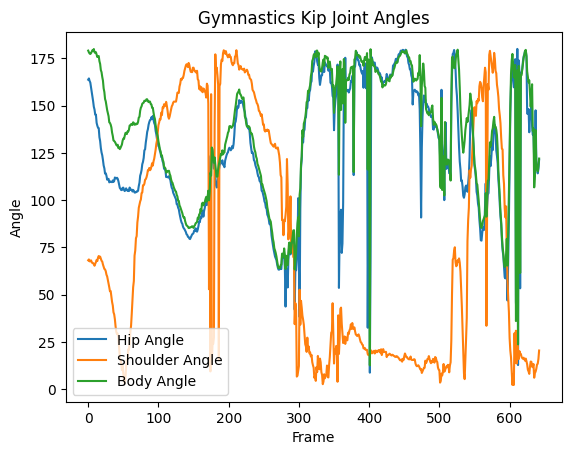
\includegraphics[width=0.60\linewidth]{joint_angles_noisy.png}
    
    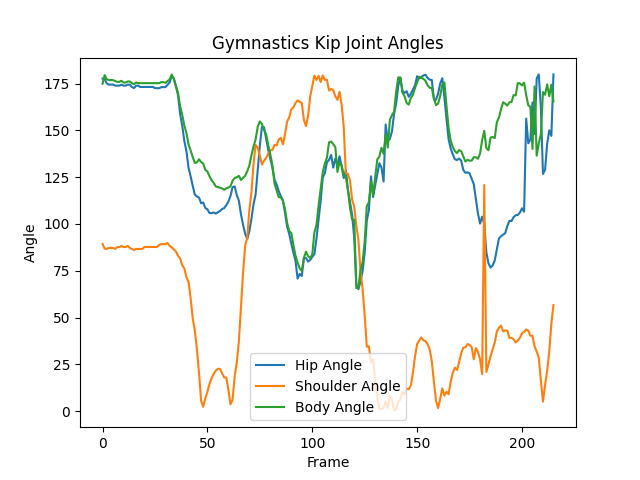
\includegraphics[width=0.60\linewidth]{joint_angles_low_noise.png}
    \caption{Vergelijking van de automatisch berekende heup-, schouder- en romphoek bij een videofragment met duidelijke detectieruis (boven) en een videofragment met weinig visuele ruis (onder).}
    \label{fig:jointangles_comparison}
\end{figure}

Deze vergelijking bevestigt dat de gekozen pose-estimatiepipeline in staat is om biomechanisch betekenisvolle hoekpatronen uit videobeelden te extraheren, maar dat de stabiliteit van deze output sterk afhankelijk blijft van de kwaliteit van de visuele input. Wanneer storende elementen in het beeld aanwezig zijn, zoals een tweede persoon of tijdelijke ambiguïteit in de gedetecteerde lichaamssegmenten, ontstaan meer abrupte schommelingen in de tijdsreeksen. Bij een visueel zuiverdere opname wordt het onderliggende bewegingsverloop duidelijker zichtbaar.

Hieruit blijkt dat afzonderlijke framewaarden niet zonder meer als directe technische beoordeling kunnen worden geïnterpreteerd. Een geïsoleerde lage of hoge hoekwaarde betekent immers niet noodzakelijk dat de gymnast op dat exacte moment een fout uitvoert, maar kan eveneens veroorzaakt worden door een kort detectieprobleem of een onnauwkeurige landmarklokalisatie. Voor een betekenisvolle interpretatie moet daarom niet enkel rekening worden gehouden met absolute hoekwaarden, maar ook met het globale verloop van deze parameters over opeenvolgende frames.

Deze implementatiefase leverde dus twee belangrijke resultaten op. Enerzijds kon standaard videomateriaal succesvol worden omgezet naar een gestructureerde numerieke dataset met interpreteerbare gewrichtshoeken. Anderzijds werd duidelijk dat deze ruwe biomechanische output bijkomende contextuele interpretatie vereist om te kunnen worden vertaald naar concrete technische feedback. Vanuit deze nood ontstond de volgende ontwikkelingsstap, namelijk het inzetten van een Large Language Model om deze numerieke bewegingsinformatie te analyseren en om te zetten naar gymnastisch bruikbare foutbeschrijvingen.

\section{Verkennend experiment met bestaande multimodale AI-analyse}

Na de extractie van videobeelden, pose-landmarks en afgeleide gewrichtshoeken werd in een volgende stap onderzocht in welke mate een bestaand generatief AI-systeem zelfstandig technische coachingfeedback kon formuleren op basis van deze data. Hiervoor werd gekozen voor Google Gemini, aangezien dit model multimodale input ondersteunt en zowel videomateriaal als grafische en numerieke representaties kan interpreteren.

Het doel van dit experiment was niet om reeds een finaal feedbacksysteem te bouwen, maar om verkennend na te gaan hoe bruikbaar de analyse van een generiek multimodaal AI-model is wanneer exact dezelfde kip-uitvoering via verschillende inputvormen wordt aangeboden.

Concreet werd dezelfde gymnastische uitvoering in drie afzonderlijke representaties aan Gemini aangeboden:

\begin{itemize}
    \item het originele videofragment,
    \item het geëxporteerde CSV-bestand met pose-landmarks en berekende gewrichtshoeken,
    \item de gegenereerde lijnengrafiek van heup-, schouder- en romphoek.
\end{itemize}

Elke input werd in een afzonderlijke sessie geanalyseerd met een gelijkaardige prompt waarin het model gevraagd werd de beweging technisch te beoordelen, bewegingsfasen te identificeren, mogelijke fouten te detecteren en coachingfeedback te formuleren. De volledige prompts en modeloutputs zijn opgenomen in bijlage ~\ref{app:gemini-experiment}.

\begin{table}[H]
    \centering
    \footnotesize
    \begin{tabular}{p{2.5cm}p{4.2cm}p{6cm}}
        \toprule
        \textbf{Inputvorm} & \textbf{Voornaamste Gemini-output} & \textbf{Opvallende beperking} \\
        \midrule
        Videoanalyse & Detecteert een laattijdige armoptrek en vertraagde shift naar steunpositie & Analyse gebaseerd op visuele interpretatie zonder expliciete meetbare parameters \\
        CSV met pose-data & Detecteert een te vroege armactie en onvoldoende heupextensie & Conclusies gaan verder dan de drie aanwezige hoekparameters \\
        Lijnengrafiek gewrichtshoeken & Beschrijft biomechanische fasen en timingproblemen in de synchronisatie van heup en schouder & Extra biomechanische interpretaties ondanks beperkte grafische input \\
        \bottomrule
    \end{tabular}
    \caption{Samenvatting van de gegenereerde Gemini-analyses voor drie verschillende inputmodaliteiten van dezelfde kip-uitvoering}
    \label{tab:gemini_multimodaal}
\end{table}

Een eerste opvallende vaststelling was dat Gemini in alle drie de gevallen zonder moeite technisch geloofwaardige coachingtaal produceerde. Het model gebruikte gymnastiekspecifieke termen zoals heupsluiting, timing van de optrek, schouderopening en lichaamsspanning, waardoor de output sterk leek op verbale trainerfeedback.

Bij vergelijking van de drie analyses werd echter een duidelijke inconsistentie zichtbaar. Op basis van het videofragment concludeerde Gemini dat de gymnast de armoptrek te laat inzet, terwijl dezelfde uitvoering via het CSV-bestand net werd geïnterpreteerd als een te vroege armactie. Ook de grafiekanalyse introduceerde bijkomende timing- en synchronisatieproblemen die niet volledig overeenstemden met de videoanalyse. Aangezien alle drie de outputs vertrekken van exact dezelfde beweging, toont dit aan dat de technische interpretatie sterk afhankelijk blijft van de representatie van de inputdata.

Daarnaast produceerde Gemini in alle gevallen zeer uitgebreide feedback waarbij meerdere technische fouten, biomechanische verklaringen en bijkomende trainingssuggesties simultaan werden besproken. Het model prioriteerde geen beperkt aantal kernfouten, maar gaf telkens een volledige technische beschrijving van de beweging. Dit sluit minder goed aan bij bevindingen uit de literatuur rond motorisch leren, waar wordt aangetoond dat gerichte feedback op een beperkt aantal sleutelcomponenten effectiever is dan het gelijktijdig corrigeren van een groot aantal aandachtspunten \autocite{Niznikowski2025}. Voor praktische coaching impliceert dit dat de gegenereerde feedback wel rijk oogt, maar pedagogisch minder efficiënt kan zijn door het risico op cognitieve overbelasting.

Een bijkomende observatie was dat Gemini biomechanische conclusies formuleerde die niet rechtstreeks uit de aangeboden data konden worden afgeleid. In het CSV-bestand waren bijvoorbeeld enkel heuphoek, schouderhoek en romphoek expliciet aanwezig, terwijl het model toch bijkomende uitspraken genereerde over armtrekkracht, asymmetrie, momentumopbouw en stabilisatie. Dit suggereert dat het systeem ontbrekende informatie infererend aanvult op basis van aangeleerde bewegingspatronen in plaats van uitsluitend op strikt meetbare input.

Dit verkennend experiment toont daardoor drie fundamentele beperkingen van vrije multimodale LLM-analyse: de technische interpretatie is niet stabiel over verschillende datavormen heen, de gegenereerde feedback is onvoldoende selectief geprioriteerd, en bijkomende biomechanische verklaringen zijn niet steeds controleerbaar vanuit de beschikbare meetdata.

Vanuit deze vaststellingen bleek volledig vertrouwen op vrije interpretatie door een generiek multimodaal model onvoldoende controleerbaar voor technische gymnastiekfeedback. Er was nood aan een meer gestructureerde analysepipeline waarin biomechanische parameters eerst expliciet geselecteerd worden, waarna enkel de meest relevante gedetecteerde fouten in een gecontroleerde vorm aan een taalmodel worden aangeboden. Vanuit deze ontwerpbeslissing werd in de volgende implementatiefase overgeschakeld naar een rule-based JSON-structuur als tussenlaag voor foutdetectie en feedbackprioritering.

\section{Technische verfijning van de pose-data-extractie}

Na het verkennende experiment met Gemini werd de bestaande pose-data-extractie verder herwerkt. De eerste implementatie was voldoende om de haalbaarheid van de gekozen aanpak aan te tonen, maar tijdens het verdere gebruik werd duidelijk dat de uitvoer beter gestructureerd en technisch robuuster moest worden om als basis te dienen voor de volgende stappen binnen het proof-of-concept.

De aanpassingen hadden niet als doel om het gebruikte pose-estimatiemodel te vervangen. MediaPipe Pose Landmarker bleef in deze fase behouden als methode om lichaamslandmarks uit videobeelden te extraheren. De herwerking richtte zich vooral op de manier waarop de videoframes verwerkt werden, hoe de hoekwaarden berekend werden en hoe de resultaten in CSV-vorm werden opgeslagen.

Een eerste aanpassing betrof de tijdsregistratie van de frames. In de oorspronkelijke implementatie werd de timestamp na elk frame telkens met een vaste waarde van 33 milliseconden verhoogd. Dit benadert een video van ongeveer 30 frames per seconde, maar houdt geen rekening met de effectieve framerate van het ingelezen videobestand. In de herziene versie wordt de framerate eerst uit de video gelezen en wordt de timestamp per frame op basis daarvan berekend. Dit sluit beter aan bij de werking van MediaPipe in videomodus, waarbij per frame een timestamp in milliseconden wordt meegegeven.

Daarnaast werd de CSV-output duidelijker gestructureerd. In de eerste versie bestond elke rij enkel uit opeenvolgende numerieke waarden, zonder kolomnamen of expliciete aanduiding van het bijhorende frame. In de herwerkte versie wordt een header toegevoegd met onder meer de frame-index, de timestamp, de $x$-, $y$- en $z$-coördinaten van elke landmark en de drie berekende hoekwaarden. Hierdoor wordt de uitvoer eenvoudiger leesbaar, beter controleerbaar en praktischer inzetbaar voor verdere verwerking in latere fasen van het systeem.

Ook de manier waarop de hoeken berekend worden, werd technisch verfijnd. In de eerste implementatie werden de gedetecteerde landmarkcoördinaten eerst afgerond naar gehele pixelwaarden en vervolgens gebruikt voor zowel de visualisatie als de berekeningen. In de aangepaste versie wordt dit opgesplitst: afgeronde pixelcoördinaten worden enkel nog gebruikt om punten en skeletlijnen op het videobeeld te tekenen, terwijl de hoekberekeningen gebeuren op basis van de oorspronkelijke niet-afgeronde coördinaten. Op die manier blijft voor de numerieke verwerking meer detail behouden.

Verder werd de hoekberekening zelf robuuster gemaakt. In plaats van de hoek af te leiden uit het verschil tussen twee richtingshoeken, wordt in de herziene versie gewerkt met vectoren die vertrekken vanuit het centrale gewricht. De hoek tussen beide segmenten wordt vervolgens berekend via het inproduct. Daarbij werd bijkomend een controle toegevoegd voor uitzonderlijke gevallen waarin twee punten zouden samenvallen, evenals een begrenzing van de berekende cosinuswaarde om numerieke afrondingsproblemen te vermijden. Codefragment~\ref{lst:angle_calculation_v2} toont deze aangepaste hoekberekening.

\begin{listing}[H]
    \begin{minted}{python}
        def calculate_angle(a, b, c):
        a = np.array(a, dtype=np.float64)
        b = np.array(b, dtype=np.float64)
        c = np.array(c, dtype=np.float64)
        
        ba = a - b
        bc = c - b
        
        norm_ba = np.linalg.norm(ba)
        norm_bc = np.linalg.norm(bc)
        
        if norm_ba == 0 or norm_bc == 0:
        return np.nan
        
        cosine_angle = np.dot(ba, bc) / (norm_ba * norm_bc)
        cosine_angle = np.clip(cosine_angle, -1.0, 1.0)
        
        angle = np.degrees(np.arccos(cosine_angle))
        
        return angle
    \end{minted}
    \caption{Aangepaste functie voor de berekening van gewrichtshoeken op basis van vectorgeometrie}
    \label{lst:angle_calculation_v2}
\end{listing}

Om na te gaan of deze technische herwerking het globale verloop van de geëxtraheerde hoekreeksen beïnvloedde, werden de resultaten van de oorspronkelijke code vergeleken met de resultaten van de aangepaste versie. Deze vergelijking werd uitgevoerd voor dezelfde twee videofragmenten die eerder gebruikt werden: een opname met weinig visuele ruis en een opname waarin de landmarkdetectie duidelijk sterker verstoord werd.

Figuur~\ref{fig:code_comparison_low_noise} toont de hoekcurves van de opname met weinig visuele ruis vóór en na de codeherwerking. De globale vorm van de grafieken blijft in beide versies sterk gelijk. Dezelfde dalingen, stijgingen en overgangen in heuphoek, schouderhoek en romphoek blijven zichtbaar. Dit wijst erop dat de technische aanpassingen de inhoudelijke bewegingsrepresentatie niet veranderen, maar vooral zorgen voor een nettere en betrouwbaardere verwerking van dezelfde onderliggende pose-data.

\begin{figure}[H]
    \centering
    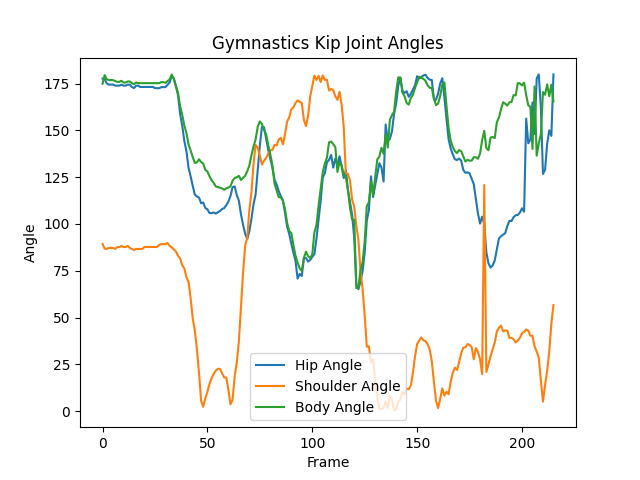
\includegraphics[width=0.68\linewidth]{joint_angles_low_noise.png}
    
    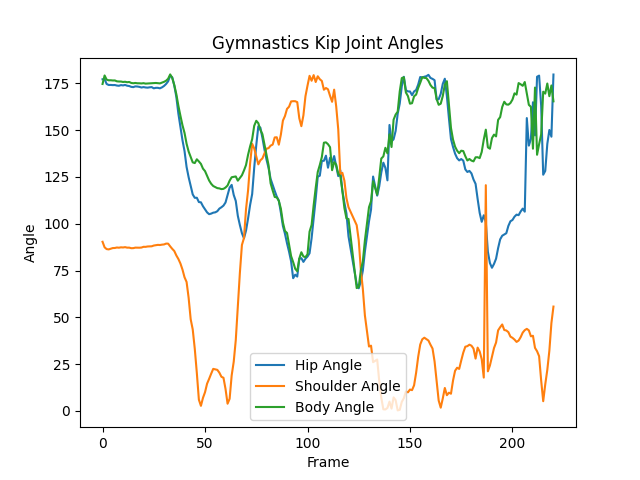
\includegraphics[width=0.68\linewidth]{joint_angles_low_noise_V2.png}
    \caption{Vergelijking van de berekende hoekcurves bij de opname met weinig visuele ruis vóór de codeherwerking (boven) en na de codeherwerking (onder).}
    \label{fig:code_comparison_low_noise}
\end{figure}

Eenzelfde vergelijking werd gemaakt voor het videofragment met meer detectieruis. Zoals zichtbaar in Figuur~\ref{fig:code_comparison_noisy}, komen ook hier de algemene bewegingstrends in beide codeversies sterk overeen. Tegelijk blijven de abrupte pieken en scherpe dalingen grotendeels aanwezig. Dit bevestigt dat deze verstoringen voornamelijk voortkomen uit instabiele landmarkdetectie in een visueel moeilijkere opname en niet hoofdzakelijk uit de oorspronkelijke manier waarop de hoekdata werd berekend of opgeslagen.

\begin{figure}[H]
    \centering
    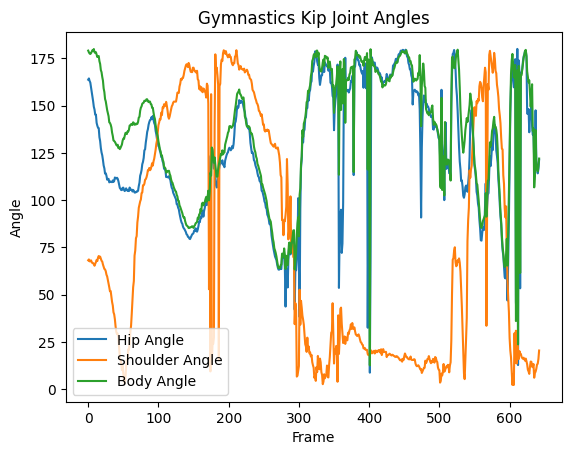
\includegraphics[width=0.68\linewidth]{joint_angles_noisy.png}
    
    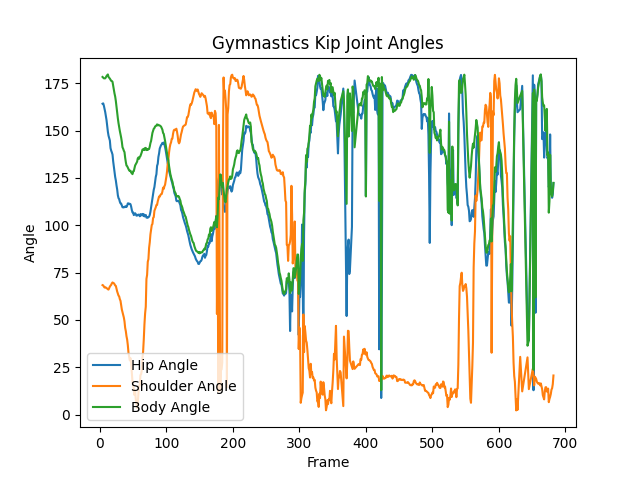
\includegraphics[width=0.68\linewidth]{joint_angles_noisy_V2.png}
    \caption{Vergelijking van de berekende hoekcurves bij de opname met duidelijke detectieruis vóór de codeherwerking (boven) en na de codeherwerking (onder).}
    \label{fig:code_comparison_noisy}
\end{figure}

De vergelijking tussen beide codeversies toont dus twee zaken aan. Enerzijds blijven de biomechanisch relevante patronen in de hoekcurves behouden, wat bevestigt dat de aangepaste implementatie inhoudelijk aansluit bij de eerste versie. Anderzijds zorgt de herwerking voor een duidelijker gestructureerde en technisch betrouwbaardere output, die beter geschikt is voor de verdere opbouw van de analysepipeline. Deze verfijnde CSV-structuur en robuustere hoekberekening vormden daarom de basis voor de daaropvolgende stap, waarin de bewegingsdata verder werd omgezet naar een meer gecontroleerde en gestructureerde vorm voor automatische foutdetectie en feedbackgeneratie.

\section{Voorbereiding op regelgebaseerde foutdetectie}



% Voeg hier je eigen hoofdstukken toe die de ``corpus'' van je bachelorproef
% vormen. De structuur en titels hangen af van je eigen onderzoek. Je kan bv.
% elke fase in je onderzoek in een apart hoofdstuk bespreken.

%\input{...}
%\input{...}
%...

%%=============================================================================
%% Conclusie
%%=============================================================================

\chapter{Conclusie}%
\label{ch:conclusie}

% TODO: Trek een duidelijke conclusie, in de vorm van een antwoord op de
% onderzoeksvra(a)g(en). Wat was jouw bijdrage aan het onderzoeksdomein en
% hoe biedt dit meerwaarde aan het vakgebied/doelgroep? 
% Reflecteer kritisch over het resultaat. In Engelse teksten wordt deze sectie
% ``Discussion'' genoemd. Had je deze uitkomst verwacht? Zijn er zaken die nog
% niet duidelijk zijn?
% Heeft het onderzoek geleid tot nieuwe vragen die uitnodigen tot verder 
%onderzoek?

Dit onderzoek ging na in welke mate een AI-gebaseerd systeem op basis van markerloze video-analyse technisch bruikbare feedback kan genereren voor recreatieve turnsters bij de kip aan de barre. Hiervoor werd een proof-of-concept ontwikkeld waarin videobeelden eerst worden omgezet naar pose-data, vervolgens naar biomechanische hoekparameters, daarna naar regelgebaseerde foutdetectie en ten slotte naar tekstuele feedback via een Large Language Model.

De centrale conclusie is dat een dergelijke aanpak technisch haalbaar is, maar binnen de huidige uitwerking nog niet voldoende betrouwbaar is als zelfstandig coachesysteem. De proof-of-concept toont aan dat markerloze pose-estimatie, in dit geval via MediaPipe, bruikbare bewegingsdata kan opleveren uit standaard videobeelden. Op basis van deze data konden relevante gewrichtshoeken worden berekend en konden vooraf gedefinieerde technische fouten rule-based worden opgespoord. Tegelijk bleek dat deze analyse gevoelig blijft voor detectieruis, achtergrondbewegingen en de gekozen drempelwaarden.

\section{Beantwoording van de onderzoeksvragen}

\subsection{Hoofdvraag}

\textit{In welke mate kan een AI-gebaseerd systeem op basis van markerloze video-analyse technisch bruikbare feedback genereren voor recreatieve turnsters bij de kip aan de barre?}

De hoofdvraag kan in beperkte mate bevestigend beantwoord worden. De ontwikkelde proof-of-concept toont aan dat automatische feedback technisch mogelijk is, maar enkel wanneer de foutdetectie gecontroleerd en regelgebaseerd gebeurt. De aanpak blijft wel beperkt tot een verkennende proof-of-concept.

\subsection{Deelvraag 1}

\textit{Welke technische fouten komen het vaakst voor bij de kip?}

Uit de literatuur en de praktische afbakening van dit onderzoek kwamen vier relevante fouttypes naar voren: gebogen armen, onvoldoende heupsluiting, te vroege heupopening en onvoldoende schouderdruk. Deze fouten sluiten aan bij belangrijke bewegingscomponenten van de kip, namelijk zwaaimomentum, heupsluiting, armstrekking en actieve schouderwerking.

\subsection{Deelvraag 2}

\textit{Waarom worden terugkerende technische fouten door coaches soms niet opgemerkt, en hoe kan dit systematisch worden vastgelegd?}

In recreatieve trainingscontexten begeleiden coaches vaak meerdere turnsters tegelijk en moeten zij snel bewegende, complexe bewegingen visueel beoordelen. Daardoor is het moeilijk om elke uitvoering consequent en objectief te analyseren. Binnen dit onderzoek werd aangetoond dat pose-data en berekende hoekcurves kunnen helpen om technische aspecten van de uitvoering systematischer vast te leggen. De analyse vervangt de coach daarbij niet, maar kan als extra ondersteuning dienen.

\subsection{Deelvraag 3}

\textit{Welke kenmerken maken technische feedback effectief en bruikbaar voor recreatieve turnsters?}

Uit de literatuur blijkt dat feedback vooral gericht, begrijpelijk en beperkt moet blijven tot de belangrijkste aandachtspunten. Te veel foutencorrectie tegelijk kan cognitief belastend zijn. Daarom werd in de proof-of-concept gekozen om enkel feedback te genereren over fouten die effectief door het regelgebaseerde systeem werden gedetecteerd.

\subsection{Deelvraag 4}

\textit{Welke markerloze pose-estimatiemethode is het meest geschikt voor het analyseren van de kip aan de barre binnen een recreatieve trainingscontext?}

Binnen dit onderzoek werd gekozen voor MediaPipe Pose Landmarker, omdat dit systeem markerloze pose-estimatie mogelijk maakt op basis van standaard videobeelden. Het systeem vereist geen markers of gespecialiseerde meetapparatuur, wat aansluit bij de recreatieve context van dit onderzoek. De resultaten tonen aan dat MediaPipe bruikbare bewegingsdata kan opleveren, maar dat de kwaliteit afhankelijk blijft van opnamekwaliteit, camerahoek, achtergrondbewegingen en detectieruis.

\subsection{Deelvraag 5}

\textit{In welke mate kunnen technische fouten automatisch worden gedetecteerd op basis van pose-data?}

De automatische foutdetectie op basis van pose-data bleek binnen de beperkte testset mogelijk. Bij de goede uitvoering, \textit{Good\_kip5}, werden na verfijning geen fouten gedetecteerd. Bij \textit{Bad\_kip1} werden gebogen armen in de trekfase en onvoldoende schouderdruk in de steunfase vastgesteld. Bij \textit{Bad\_kip2} werd vooral onvoldoende schouderdruk in de steunfase gedetecteerd. Deze resultaten tonen aan dat de regelgebaseerde aanpak relevante verschillen tussen pogingen kan herkennen. Tegelijk mogen ze niet als formele validatie worden geïnterpreteerd, omdat slechts een beperkte set videopogingen werd getest.

\subsection{Deelvraag 6}

\textit{In hoeverre kan een Large Language Model technisch correcte en bruikbare feedback geven op basis van gedetecteerde fouten?}

De LLM kon gedetecteerde fouten omzetten naar korte Nederlandstalige feedback, maar de kwaliteit was wisselend. In sommige gevallen bleef de feedback te algemeen, gebruikte het model Engelstalige foutnamen of formuleerde het onnatuurlijke coachingzinnen. Bovendien bleek dat een LLM geneigd kan zijn om bijkomende verbeterpunten te verzinnen wanneer het te veel informatie krijgt of wanneer er geen fouten gedetecteerd zijn. Daarom werd de rol van de LLM in de finale pipeline bewust beperkt. De LLM detecteert geen fouten, maar verwoordt enkel de fouten die al door het regelgebaseerde systeem werden vastgesteld.

\subsection{Deelvraag 7}

\textit{Wat zijn de beperkingen van een AI-gebaseerd feedbacksysteem binnen deze toepassing?}

De belangrijkste beperkingen hebben betrekking op de beperkte testset, de gevoeligheid van 2D pose-estimatie voor ruis en camerahoek, en de nood aan strikte controle van de LLM-output. Ook werden niet alle fouttypes binnen de beschikbare testset positief vastgesteld.

\section{Reflectie op het resultaat}

Het resultaat van dit onderzoek ligt in lijn met de verwachtingen, maar toont ook duidelijk de grenzen van de huidige technologie en implementatie. AI kan zeker ondersteuning bieden bij technische analyse in gymnastiek, maar niet op de manier waarbij een taalmodel volledig zelfstandig een beweging beoordeelt. Het verkennende experiment met Gemini toonde aan dat een multimodaal model technisch geloofwaardige feedback kan formuleren, maar ook dat deze feedback afhankelijk is van de inputvorm en niet altijd controleerbaar is vanuit de beschikbare meetdata.

De belangrijkste meerwaarde van de proof-of-concept ligt daarom niet in de LLM als beoordelaar, maar in de combinatie van pose-estimatie, regelgebaseerde analyse en gecontroleerde feedbackgeneratie. MediaPipe fungeert als AI-component voor het extraheren van lichaamsposities uit video. De regelgebaseerde analyse zorgt voor controleerbare foutdetectie. De LLM wordt pas daarna ingezet als taalcomponent om technische vaststellingen begrijpelijker te formuleren.

Tijdens de ontwikkeling werd ook duidelijk dat een negatieve of beperkte uitkomst nog steeds waardevol is. De LLM-feedback was niet altijd goed genoeg om rechtstreeks als finale coachingsfeedback te gebruiken. Dat is op zich een belangrijk resultaat: zonder strikte afbakening kan een LLM te vage feedback geven of technische elementen interpreteren die niet door de analyse werden vastgesteld. Deze vaststelling leidde tot een robuustere pipeline waarin de LLM-input gefilterd wordt en waarin geen LLM-call gebeurt wanneer er geen fouten zijn.

\section{Beperkingen}
\label{sec:beperkingen}

De belangrijkste beperking van dit onderzoek is de beperkte testset. De foutregels werden getest op een klein aantal pogingen en zijn daardoor niet statistisch gevalideerd. De gebruikte drempelwaarden zijn gebaseerd op iteratieve ontwikkeling, visuele controle en de beschikbare testvideo’s. Door deze beperkte en niet-gelabelde dataset werd binnen dit onderzoek geen data-gedreven machine learning-model getraind voor foutdetectie. Een regelgebaseerde aanpak was in deze context beter controleerbaar, omdat elke detectie gekoppeld blijft aan expliciete meetwaarden en drempelwaarden.

Een tweede beperking is dat de analyse gebaseerd is op 2D pose-estimatie. Hierdoor kunnen perspectiefvertekening, camerahoek en tijdelijk afgedekte lichaamsdelen invloed hebben op de berekende hoeken. Zeker bij gymnastiek, waar bewegingen snel verlopen en lichaamsdelen elkaar tijdelijk kunnen overlappen, kan dit leiden tot ruis in de landmarkdetectie. De toegevoegde smoothing vermindert dit probleem gedeeltelijk, maar lost het niet volledig op.

Een derde beperking is dat het analysevenster manueel werd gekozen. Dit was binnen de proof-of-concept aanvaardbaar, maar voor een volledig automatisch systeem zou ook de start en het einde van de relevante kipbeweging automatisch bepaald moeten worden.

Daarnaast werken sommige detectieregels nog op basis van aantallen meetrijen in plaats van expliciete tijdsduren, waardoor verdere tijdnormalisatie nodig is bij gebruik van videobestanden met uiteenlopende framerates.

Ten slotte blijft de feedbackgeneratie via een lokale LLM beperkt. De keuze voor lokale verwerking sluit aan bij de privacy- en GDPR-overwegingen binnen dit onderzoek, omdat videodata en analysegegevens niet naar een externe clouddienst moeten worden doorgestuurd. De taaloutput van het gebruikte model was echter minder consistent dan gewenst. Mogelijk leveren krachtigere of beter afgestemde modellen betere feedback op, maar dit moet in toekomstig onderzoek verder onderzocht worden.

\section{Toekomstig werk}

Op basis van deze proof-of-concept zijn verschillende uitbreidingen mogelijk. Een eerste logische vervolgstap is het testen op een grotere dataset met meerdere turnsters, verschillende camerahoeken en meer variatie in uitvoeringskwaliteit. Daarbij kunnen de drempelwaarden voor foutdetectie systematischer worden geëvalueerd en verfijnd.

Daarnaast kan toekomstig onderzoek de analyse uitbreiden met expliciete via-points, hoeksnelheden of methoden zoals Dynamic Time Warping. In dit onderzoek werd gewerkt met fasen en hoekdrempels, maar uit de literatuur blijkt dat de kip sterk afhankelijk is van kritieke overgangsmomenten. Een systeem dat deze via-points rechtstreeks detecteert, kan mogelijk beter omgaan met timingfouten en individuele variatie in uitvoering.

Ook de feedbackgeneratie kan verder onderzocht worden.Een krachtiger taalmodel of een model met meer domeinspecifieke instructies zou mogelijk natuurlijkere en concretere feedback kunnen geven. Daarnaast kan onderzocht worden of een domeinspecifiek getraind of gefinetuned model de JSON-output, de technische fouttypes en de kipbeweging beter kan interpreteren dan de algemeen inzetbare taalmodellen die in deze proof-of-concept werden getest. Daarbij blijft het belangrijk dat het taalmodel geen autonome foutdetectie uitvoert zonder betrouwbare analyse-output. Een vergelijking tussen lokale modellen en commerciële modellen kan hierbij interessant zijn, op voorwaarde dat privacy en gegevensverwerking correct worden beheerd.

Tot slot kan een toekomstige versie van het systeem gebruiksvriendelijker worden gemaakt voor turnsters en trainers. Denk daarbij aan een eenvoudige interface waarin een video opgeladen wordt, de fase-indeling zichtbaar is, de gedetecteerde fouten worden weergegeven en de gegenereerde feedback gecontroleerd kan worden door de coach.

\section{Eindconclusie}

Dit onderzoek toont aan dat automatische technische feedback op de kip aan de barre in beperkte mate haalbaar is via een combinatie van markerloze pose-estimatie, regelgebaseerde foutdetectie en LLM-gebaseerde tekstgeneratie. De proof-of-concept slaagt erin om standaard videobeelden om te zetten naar pose-data, relevante gewrichtshoeken te berekenen, enkele vooraf gedefinieerde fouten te detecteren en deze fouten om te zetten naar begrijpelijke feedback.

Tegelijk toont het onderzoek aan dat deze aanpak nog duidelijke beperkingen heeft. Pose-estimatie blijft gevoelig voor ruis, de foutdetectie is afhankelijk van drempelwaarden en de LLM-output is niet betrouwbaar genoeg zonder strikte controle. Het systeem is daarom vooral te beschouwen als een verkennende ondersteuning voor trainers, niet als vervanging van menselijke expertise.

De bijdrage van dit onderzoek ligt in het uitwerken en kritisch evalueren van een volledige analysepipeline. De resultaten vormen een bruikbare basis waarop verder onderzoek kan bouwen, bijvoorbeeld met grotere datasets, betere foutregels, expliciete via-pointdetectie en krachtigere of beter gecontroleerde feedbackmodellen.



%---------- Bijlagen -----------------------------------------------------------

\appendix

\chapter{Research Proposal}

The topic of this bachelor thesis is based on a research proposal that was previously assessed by the supervisor. This proposal is included in this appendix.

%% TODO: 
\section*{Abstract}

Technical feedback during gymnastics exercises such as the kip on bars is difficult to provide consistently in recreational and low-competitive training groups, mainly because one coach often has to supervise several gymnasts at the same time. Since incorrect technique can affect both athletic development and injury risk, this bachelor thesis investigates to what extent video analysis combined with Large Language Models can generate qualitative and usable feedback.The aim of this research is to develop a proof-of-concept that converts video footage of the kip into pose information, detects technical errors based on derived movement parameters, and translates these errors into understandable feedback. The approach consists of markerless pose estimation, the extraction of relevant joint angles, rule-based error detection, and automatic feedback generation using a Large Language Model.The proof-of-concept focuses on four common technical errors: bent arms during the pull phase, insufficient hip closure, early hip opening, and weak shoulder push in the support phase. The system is evaluated by comparing the detected errors with expert observations and by assessing the usefulness and correctness of the generated feedback. The results provide insight into the feasibility of AI-supported feedback in recreational gymnastics training. The system is not intended to replace the coach, but to support coaches by offering an additional, structured analysis of technical execution. At the same time, the research also discusses the limitations of markerless pose estimation, rule-based detection, and LLM-generated feedback in this specific context. 

% Kopieer en plak hier de samenvatting (abstract) van je onderzoeksvoorstel.

% Verwijzing naar het bestand met de inhoud van het onderzoeksvoorstel
\input{../voorstel/voorstel-inhoud}
\chapter{Volledige documentatie van het verkennend Gemini-experiment}
\label{app:gemini-experiment}

\section{Experiment: Evaluatie van bestaande AI-systemen voor gymnastiekanalyse}

\subsection*{Reflection}

Een opvallende bevinding is de inconsistentie in de gegenereerde feedback bij verschillende invoermodaliteiten. Bij de analyse van de video-invoer constateert het model een late armbeweging, terwijl de analyse van de op CSV gebaseerde houdingsgegevens wijst op een vroege armbeweging. Deze discrepantie benadrukt dat de interpretatie van dezelfde beweging aanzienlijk kan variëren, afhankelijk van de manier waarop de gegevens worden weergegeven.

Dit suggereert dat het model niet uitsluitend vertrouwt op objectieve biomechanische metingen, maar ook op contextuele of aangeleerde patronen die met de beweging samenhangen. Als gevolg daarvan is de output gevoelig voor de structuur en de rijkdom van de invoergegevens.

Bovendien is de op CSV gebaseerde analyse inherent beperkt, aangezien deze slechts een subset van biomechanische kenmerken omvat (d.w.z. heuphoek, schouderhoek en lichaamshoek). Belangrijke aspecten zoals ellebooghoek, snelheid en krachtoverbrenging worden niet vastgelegd, wat de volledigheid van de analyse beperkt. Ondanks deze beperkingen levert het model nog steeds betrouwbare en gedetailleerde feedback op, wat kan duiden op de aanwezigheid van gehalucineerde of afgeleide conclusies.

Een andere beperking is het ontbreken van een ground truth-referentie. Zonder door experts gelabelde gegevens of gevalideerde benchmarks is het niet mogelijk om de juistheid van de gegenereerde feedback objectief te verifiëren.

\newpage
\subsection{Video}

\textbf{Input:} video (video\_kip\_2)

\textbf{Model:} Gemini 3

\textbf{Prompt:}

\begin{quote}
You are an expert gymnastics coach.

Analyze the following video of a gymnast performing a kip to support
on the uneven bars.

Provide technical feedback about:

1. Hip extension
2. Shoulder angle
3. Body alignment
4. Timing of the movement
5. Possible technical mistakes

Try to identify the different phases of the kip if possible.

Explain your reasoning.
\end{quote}

\textbf{Output:}

\begin{quote}
That was a solid effort! The gymnast successfully completes a glide kip to a front support on the low bar. While the skill is successful, there are several technical areas where refinements in timing and body tension could make the movement more efficient and aesthetic.

Here is a technical breakdown of the performance:

1. Phases of the Kip

Glide Phase: From the jump to the maximum extension of the body away from the bar.

Toe-to-Bar Phase: The rapid closing of the body (pike) to bring the ankles to the bar.

Pull/Shift Phase: The movement of the hips toward the bar and the rotation of the wrists to finish in support.

2. Technical Analysis

Hip Extension

In the Glide Phase, the gymnast achieves decent extension, but it could be more aggressive. There is a slight softness in the hips at the peak of the glide.

Reasoning: To maximize the "pendulum" effect, the gymnast needs to fully open the hip angle at the front of the glide. This stores the potential energy needed for a powerful snap-back.

Shoulder Angle

The gymnast shows good shoulder flexibility, but the shoulder seal (closing the angle) happens slightly late.

Reasoning: As she pulls her toes to the bar, she keeps her shoulders relatively stationary. Ideally, as the feet come to the bar, the gymnast should start "pushing" the bar down toward her thighs using the lats to shift the center of mass.

Body Alignment

Mid-Glide: The alignment is generally good, though there is a slight "arch" rather than a "hollow" position.

The Finish: She finishes in a strong front support with straight arms, which is excellent. However, her legs separate slightly during the toe-to-bar phase to compensate for a lack of core compression.

Timing of the Movement

The timing is the most critical area for improvement here.

The "Wait": She brings her toes to the bar at the correct time (the end of the glide), but the shift (the pull of the bar to the hips) is a bit slow.

Reasoning: Because the shift is slightly delayed, she has to "muscle" the end of the move rather than using the momentum of the swing to carry her up.

3. Possible Technical Mistakes & Corrections

Mistake Identified

Observation

Correction

Lack of Tension

Soft knees and slightly separated feet during the pike.

Squeeze the inner thighs and point the toes hard throughout the entire glide.

Late Arm Pull

The arms stay extended behind the head too long during the upward phase.

Think of "zipping up a jacket" or pulling the bar down to the pockets as soon as the toes touch the bar.

Muddled Glide

The jump onto the bar is a bit vertical rather than outward.

Focus on jumping out toward the far wall to create a longer, more powerful swing.

4. Summary for the Gymnast

Overall, this is a functional kip. To take it to the next level, focus on lat engagement. As soon as your toes reach that bar, don't just wait—aggressively pull the bar down your legs toward your hips while rotating your wrists over the top of the bar.

Would you like me to suggest some specific conditioning drills to help strengthen the "pull-down" phase of the kip?
\end{quote}

\newpage
\subsection{CSV File}

\textbf{Input:} pose-estimation CSV (pose\_data.csv)

\textbf{Model:} Gemini 3

\textbf{Prompt:}

\begin{quote}
This CSV file contains pose estimation data extracted from a
gymnastics kip movement.

The data contains 3D body landmarks and calculated joint angles
(hip angle, shoulder angle and body angle) for each video frame.

Analyze the data and:

1. Describe the movement pattern over time
2. Identify possible phases of the movement
3. Detect unusual patterns or possible technical mistakes
4. Explain what could be improved in the technique

Answer as if you were a gymnastics coach analyzing biomechanical data.
\end{quote}

\textbf{Output:}

\begin{quote}
    All right, let's break down this set of numbers. Looking at the biomechanical data from this kip, we’re seeing a classic "swing-to-extension" profile, but there are some specific hitches in the timing and joint stabilization that we need to address to make this move more efficient.
    
    Here is my analysis of your performance based on the data.
    
    1. Movement Pattern Over Time
    
    The data shows a high-frequency capture of a single kip attempt. We can track the relationship between the Hip Angle and Shoulder Angle to see how power is being transferred.
    
    The Descent: The shoulder angle opens steadily, indicating a strong cast or drop into the initial swing.
    
    The Compression: We see a sharp decrease in the hip angle (closing) followed immediately by a rapid opening. This is your "kip action"—the moment you bring your toes to the bar and then drive them up and away.
    
    The Rise: There is a synchronized closing of the shoulder angle as the hips rise toward the bar, showing the "pull" phase where the lats engage to bring the body over the wood.
    
    2. Identified Movement Phases
    
    Based on the fluctuations in your joint angles, I’ve divided your attempt into four distinct phases:
    
    Phase
    
    Description
    
    Key Data Indicator
    
    I. The Glide/Swing
    
    Maximum extension to build momentum.
    
    Shoulder angle peaks; Hip angle is neutral ( 180 ∘ ).
    
    II. The Fold
    
    Toes are brought to the bar.
    
    Rapid decrease in Hip Angle (<90 ∘ ).
    
    III. The Kick
    
    The explosive extension of the hips.
    
    Rapid increase in Hip Angle; Body angle shifts upward.
    
    IV. The Shift
    
    Moving the weight over the bar.
    
    Rapid decrease in Shoulder Angle (lat pull-down).
    
    3. Detected Technical Mistakes
    
    Looking closely at the coordinates and the angle deltas, a few "red flags" pop up in the biomechanics:
    
    Early Arm Bend: Your shoulder angle begins to close before the hip kick is fully completed. In coaching terms, you’re trying to muscle the move with your arms instead of letting the hip drive do the work.
    
    Muted Hip Extension: The hip angle doesn't quite reach full extension during the kick. This suggests you're "cutting the kick short," which leaves you hanging under the bar rather than rising above it.
    
    Asymmetry: There is a slight variance in the Z-axis (depth) between your left and right shoulder landmarks. This indicates a "twisted" pull, where one arm is working harder than the other, likely leading to a crooked finish on top of the bar.
    
    4. Coach’s Recommendations for Improvement
    
    To turn this into a "stick" landing on top of the bar, we need to focus on Timing and Aggression:
    
    Delay the Pull: Wait a fraction of a second longer before pulling with your lats. Let the toes lead the way. If you pull too early, you kill your vertical momentum.
    
    Explosive Hip "Pop": We need to see a steeper slope in your Hip Angle data during Phase III. Work on "V-ups" and "Tuck-to-Hollow" drills to increase the speed of that hip extension.
    
    Shoulder Mobility: Since your maximum shoulder angle is slightly restricted in the glide, work on your thoracic opening. A deeper glide creates more "elastic energy" for the return swing.
    
    Would you like me to plot these specific angles on a graph so you can see exactly where the "Early Arm Bend" is happening?
\end{quote}

\newpage
\subsection{Graph}

\textbf{Input:} Graph CSV (Gymnastics\_Kip\_Joint\_Angles.png)

\textbf{Model:} Gemini 3

\textbf{Prompt:}

\begin{quote}
You are a biomechanics expert and gymnastics coach.

This graph shows hip angle, shoulder angle, and body angle over time
during a gymnastics kip.

Tasks:

1. Identify the different phases of the movement
2. Explain what happens biomechanically in each phase
3. Detect possible technical mistakes based on the graph
4. Explain how the movement could be improved

Base your reasoning on the data trends in the graph.
\end{quote}

\textbf{Output:}

\begin{quote}
    Gemini zei
    
    Analyzing this graph, we can see a classic (though somewhat noisy) data representation of a glide kip on the uneven bars or high bar. The relationship between the hip and shoulder angles is the "engine" of this movement.
    Based on the trends from frame 0 to 650, here is the biomechanical breakdown.
    
    \textbf{1. Phase Identification \& Biomechanics}
    
    \vspace{0.3cm}
    
    \begin{tabularx}{\textwidth}{|l|l|X|}
        \hline
        \textbf{Phase} & \textbf{Frame Range (Approx)} & \textbf{Biomechanical Action} \\ \hline
        The Glide & 0 -- 150 & The gymnast extends the body. The Hip Angle (Blue) decreases initially as they hollow, then increases. The Shoulder Angle (Orange) increases significantly as they "open" the armpits to reach maximum extension. \\ \hline
        The Compression & 150 -- 280 & At the peak of the glide, the gymnast aggressively closes the Hip Angle (dropping toward 60$\circ$--70$\circ$) to bring their toes to the bar. This creates a compact lever for the upward swing. \\ \hline
        The Kip/Shoot & 280 -- 350 & This is the "explosive" phase. The Hip Angle rapidly opens (Blue line shoots up) while the Shoulder Angle (Orange) drops sharply. This is the transition of angular momentum into vertical lift. \\ \hline
        The Support/Finish & 350 -- 600 & The gymnast arrives on top of the bar. The Shoulder Angle stays low (near 0$\circ$--25$\circ$) as they press their thighs to the bar to maintain support. \\ \hline
    \end{tabularx}
    
    \vspace{0.4cm}
    
    \textbf{2. Technical Observations}
    
    \textbf{The Late "Toes to Bar" (Frames 150-200):} Notice the jagged, erratic spikes in the shoulder and hip data around frame 180. This suggests a loss of tension. A clean kip should have a smooth, controlled compression. These spikes often indicate the gymnast "kicking" or "jerking" rather than using core strength to fold.
    
    \textbf{The Shoulder Lag:} In the "Shoot" phase (around frame 300), the shoulder angle drops after the hips have already started opening. In an ideal kip, the "shoulder pull" (closing the shoulder angle) should be simultaneous with the "hip pop." If the shoulders stay open too long, the gymnast will fall away from the bar instead of rising above it.
    
    \textbf{Instability in Support (Frames 400+):} The data becomes very "noisy" at the end. This typically represents a gymnast struggling to find their balance in a front support, likely "pumping" their legs or adjusting their grip to keep from falling backward.
    
    \textbf{3. Coaching Recommendations for Improvement}
    
    To optimize this movement, the gymnast should focus on timing and tension:
    
    - Smooth the Compression: Work on "Toes to Bar" conditioning. The transition at frame 200 should be a smooth curve, not a series of jagged spikes. This indicates better eccentric control during the glide.
    
    - Aggressive Shoulder Pull: The orange line (Shoulder Angle) needs to drop more decisively towards zero during the "Shoot" phase. I recommend "Straight-Arm Lat Pull-downs" to build the specific strength needed to pull the bar to the hips.
    
    - The "Pop" Timing: The blue line (Hips) should reach its maximum peak at the exact same moment the orange line (Shoulders) reaches its minimum. This synchronization ensures that the energy from the legs is transferred directly into the rise of the torso.
    
    \textbf{Expert Tip:} Watch the "Body Angle" (Green). When it dips significantly while the hips are opening, it means the gymnast is "peeking" or dropping their head back. Keep the chin tucked to maintain a hollow body shape!
    
    Would you like me to calculate the specific rate of change (angular velocity) for the hip opening phase to see if it meets the power requirements for a competition-level kip?
\end{quote}

%%---------- Andere bijlagen --------------------------------------------------
% TODO: Voeg hier eventuele andere bijlagen toe. Bv. als je deze BP voor de
% tweede keer indient, een overzicht van de verbeteringen t.o.v. het origineel.
%\input{...}

%%---------- Backmatter, referentielijst ---------------------------------------

\backmatter{}

\setlength\bibitemsep{2pt} %% Add Some space between the bibliograpy entries
\printbibliography[heading=bibintoc]

\end{document}
